

\section{OpticalElement: \textquotedbl{}MICADO\_SPEC\textquotedbl{}%
  \label{opticalelement-micado-spec}%
}

\textbf{Element}: instrument

\textbf{Alias}: INST

\textbf{Description}: MICADO SPEC mode effects


\subsection{Global properties%
  \label{global-properties}%
}

\begin{quote}
\begin{alltt}
\begin{lstlisting}[frame=single]
         psf : \{'wavelength': '!INST.filter_name', 'strehl': 0.4\}
    aperture : \{'x': 0, 'y': 0, 'width': 3, 'height': 0.05\}
element_name : MICADO_SPEC
\end{lstlisting}
\end{alltt}
\end{quote}


\subsection{Effects%
  \label{effects}%
}

Summary of Effects included in this optical element:

\setlength{\DUtablewidth}{\linewidth}
\begin{longtable*}[c]{|p{0.135\DUtablewidth}|p{0.286\DUtablewidth}|p{0.265\DUtablewidth}|p{0.102\DUtablewidth}|p{0.167\DUtablewidth}|}
\hline
\textbf{%
element
} & \textbf{%
name
} & \textbf{%
class
} & \textbf{%
included
} & \textbf{%
z\_orders
} \\
\hline
\endfirsthead
\hline
\textbf{%
element
} & \textbf{%
name
} & \textbf{%
class
} & \textbf{%
included
} & \textbf{%
z\_orders
} \\
\hline
\endhead
\multicolumn{5}{c}{\hfill ... continued on next page} \\
\endfoot
\endlastfoot

MICADO\_SPEC
 & 
micado\_adjustable\_slit
 & 
RectangularApertureMask
 & 
True
 & 
{[}80, 280, 380{]}
 \\
\hline

MICADO\_SPEC
 & 
spectral\_trace\_3000x50mas
 & 
SpectralTraceList
 & 
True
 & 
{[}70, 270{]}
 \\
\hline
\end{longtable*}
\label{tbl-micado-spec}


\subsubsection{RectangularApertureMask: \textquotedbl{}micado\_adjustable\_slit\textquotedbl{}%
  \label{rectangularaperturemask-micado-adjustable-slit}%
}

\textbf{Included by default}: \texttt{True}

\textbf{File Description}:

\textbf{Class Description}: <no docstring>

\textbf{Changes}:

\begin{itemize}
\item \end{itemize}


\paragraph{Data%
  \label{data}%
}
\leavevmode
\setlength{\DUtablewidth}{\linewidth}
\begin{longtable*}[c]{|p{0.098\DUtablewidth}|p{0.098\DUtablewidth}|}
\hline
\textbf{%
x
} & \textbf{%
y
} \\
\hline
\endfirsthead
\hline
\textbf{%
x
} & \textbf{%
y
} \\
\hline
\endhead
\multicolumn{2}{c}{\hfill ... continued on next page} \\
\endfoot
\endlastfoot

-1.5000
 & 
-0.0250
 \\
\hline

1.5000
 & 
-0.0250
 \\
\hline

1.5000
 & 
0.0250
 \\
\hline

-1.5000
 & 
0.0250
 \\
\hline
\end{longtable*}
\label{tbl-micado-adjustable-slit}


\paragraph{Meta-data%
  \label{meta-data}%
}

\begin{quote}
\begin{alltt}
\begin{lstlisting}[frame=single]
             filename : None
                 name : micado_adjustable_slit
                  psf : \{'wavelength': 'Ks', 'strehl': 0.4\}
             aperture : \{'x': 0, 'y': 0, 'width': 3, 'height': 0.05\}
         element_name : MICADO_SPEC
                width : !INST.aperture.width
               height : !INST.aperture.height
                    x : !INST.aperture.x
                    y : !INST.aperture.y
              z_order : [80, 280, 380]
              include : True
          pixel_scale : !INST.pixel_scale
              no_mask : True
                angle : 0
                shape : rect
       conserve_image : True
                   id : 0
  report_plot_include : False
 report_table_include : True
report_table_rounding : 4
               x_unit : arcsec
               y_unit : arcsec
\end{lstlisting}
\end{alltt}
\end{quote}


\subsubsection{SpectralTraceList: \textquotedbl{}spectral\_trace\_3000x50mas\textquotedbl{} : 1 traces%
  \label{spectraltracelist-spectral-trace-3000x50mas-1-traces}%
}

\textbf{Included by default}: \texttt{True}

\textbf{File Description}:

\textbf{Class Description}: List of spectral trace geometries for the detector plane

\textbf{Changes}:

\begin{itemize}
\item \end{itemize}


\paragraph{Data%
  \label{id1}%
}

\begin{figure}[H]
\noindent\makebox[\linewidth][c]{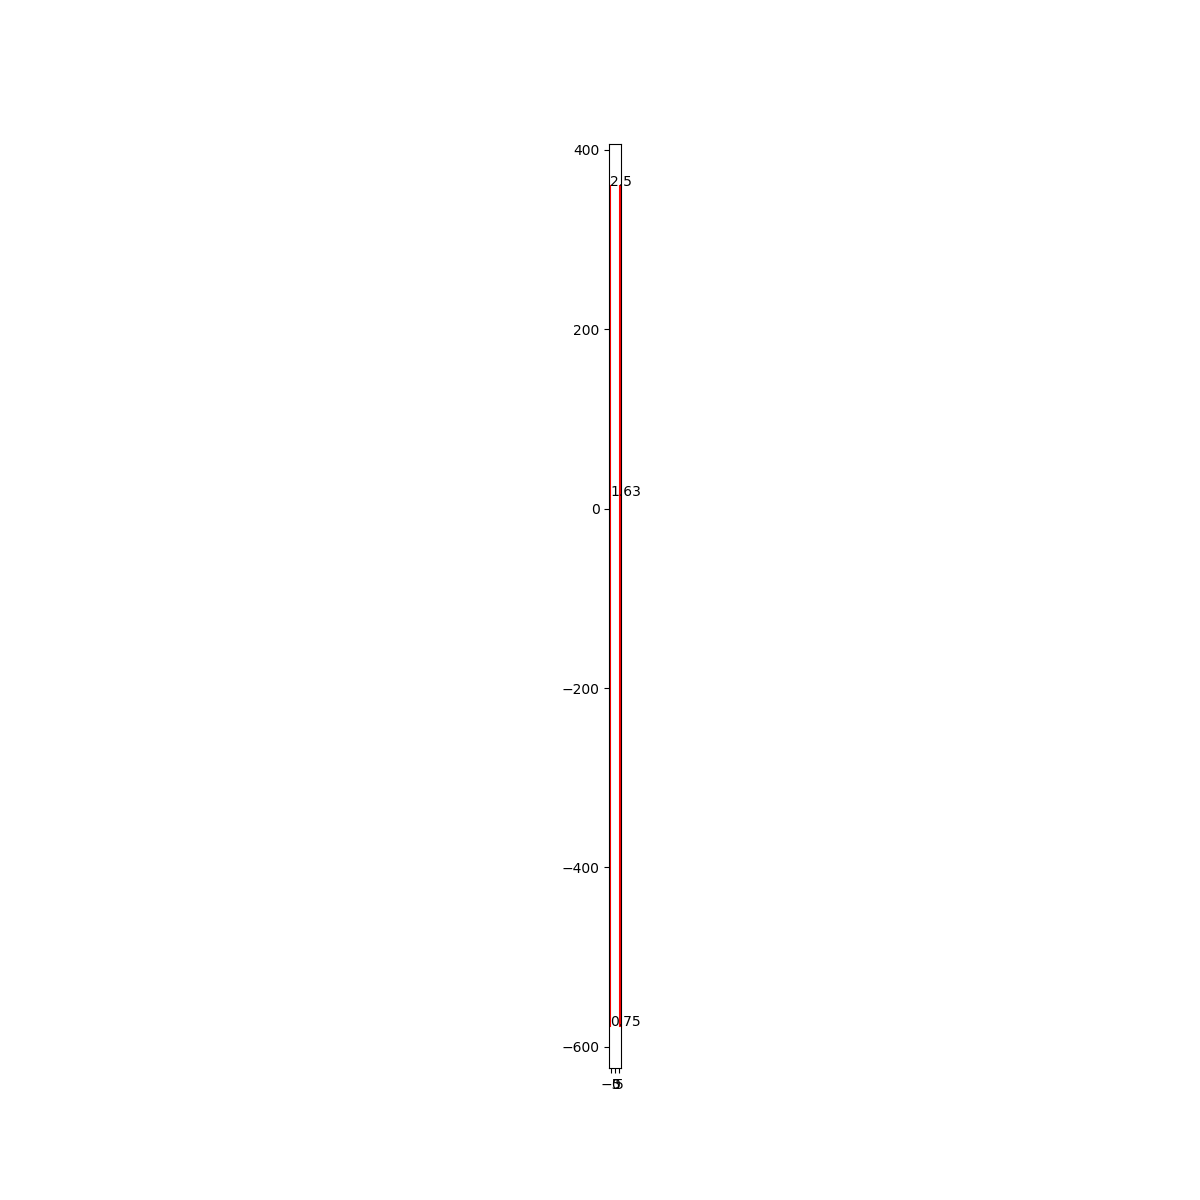
\includegraphics{spectral_trace_3000x50mas.png}}\phantomsection\label{fig-spectral-trace-3000x50mas}
\end{figure}


\paragraph{Meta-data%
  \label{id2}%
}

\begin{quote}
\begin{alltt}
\begin{lstlisting}[frame=single]
            filename : TRACE_SCI_3arcsec.fits
                name : spectral_trace_3000x50mas
                 psf : \{'wavelength': 'Ks', 'strehl': 0.4\}
            aperture : \{'x': 0, 'y': 0, 'width': 3, 'height': 0.05\}
        element_name : MICADO_SPEC
  center_on_wave_mid : True
              SIMPLE : True
              BITPIX : 8
               NAXIS : 0
              EXTEND : True
                ECAT : 1
               EDATA : 2
             z_order : [70, 270]
             include : True
         pixel_scale : !INST.pixel_scale
         plate_scale : !INST.plate_scale
            wave_min : !SIM.spectral.wave_min
            wave_mid : !SIM.spectral.wave_mid
            wave_max : !SIM.spectral.wave_max
           x_colname : x
           y_colname : y
           s_colname : s
        wave_colname : wavelength
    col_number_start : 0
               dwave : 0.002
       invalid_value : None
 report_plot_include : True
report_table_include : False
\end{lstlisting}
\end{alltt}
\end{quote}
